\newcommand{\pCount}{24 }
\section{User-Centered Evaluation}

We conduct a user study to evaluate the effectiveness of our approach. We chose this type of evaluation because legibility is a human-centred characteristic. Many different types of statistical error metrics have been evaluated in previous work \cite{nusrat2016State}, however, our focus is more user-centric in nature.

\subsection{Study Hypothesis}

We formulate the following hypotheses to motivate our user study:

\textbf{H1:} The introduction of rivers can improve the legibility and recognizability of cartograms.

\textbf{H1.1:} The introduction of rivers can increase the accuracy of the target location.

\textbf{H1.2:} The introduction of rivers can reduce the time required to locate a target region in a cartogram.

We test these hypotheses using location-based tasks. Given a standard choropleth on the left side of the screen and the equivalent cartogram on the right side, we ask user study participants to locate the given region in the choropleth (on the left) in the cartogram (on the right). See \Cref{fig:task}.

\subsection{User Study Variables}

In this section, we discuss the variables of our user study.

\bobgraph{Independent Variables: }The primary independent variable is the presence of rivers in the cartograms, which directly impacts the final layout of the cartogram. We set this parameter to render rivers or not.

% {
% \renewcommand{\arraystretch}{1.5}
% \begin{table}[!tb]
% 	\centering
% 		\begin{tabulary}{\columnwidth}{|*{2}{c|}}
% 			\hline
% 			\cellcolor{Mycolor2}\textbf{River Crossing} &
% 			\cellcolor{Mycolor2}\textbf{River Presence} \\
% 			\hline
% 			Allow & Present \\
% 			\hline
% 			Allow & Absent \\
% 			\hline
% 			Disallow & Present \\
% 			\hline
% 			Disallow & Absent \\
% 			\hline
% 		\end{tabulary}
% 	\caption{The combinations of independent variables.}
% 	\label{table:Independent Variables}
% \end{table}
% }


\bobgraph{Dependent Variables: }\textit{Accuracy:} Given a CCG location in the choropleth on the left, we ask the participant to locate the corresponding node in the cartogram. Accuracy as the primary dependent variable is measured by the number of correct CCGs located and chosen by the participants. \textit{Response time:} Another dependent variable is the time it takes the participants to complete each task.

\bobgraph{Control Variables: }\textit{Choice of color map:} We use D3's built-in interpolateRdYlGn color map, a diverging color scheme of red, yellow, and green, to depict the data in our cartograms. \textit{Communicating the target CCG to the user:} We inform the participant about the target CCG they need to find. The target CCG is shown in the form of a nonstop blinking (between its original color and black) area on the screen, each blink is given a duration of 2 seconds.

\subsection{User Study Design}
In this section we describe the user study participants, datasets, and the experimental procedure.

\bobgraph{Participants:} We recruited \pCount participants.

\begin{itemize}
    \item Gender: 10 females and 14 males
    \item Age Group: 18-24 (16), 25-29 (8)
    \item Education: 1 PhD, 11 Master's, 8 Bachelor's, 4 Others
\end{itemize}

\bobgraph{Datasets:} We used the following EHR datasets for our evaluation:

\begin{itemize}
    \item Population
    \item Under 75 mortality from cardiovascular disease
    \item Emergency admissions for alcohol-related liver disease
    \item Alcohol-specific admission and readmission
\end{itemize}

135 CCGs are rendered on the screen as a choropleth on the left. We then generated another view on the right using cartograms. The color of both visual designs is mapped to the dataset. See \Cref{fig:task} for an example.

    {
        \begin{figure}[tb!]
            \centering
            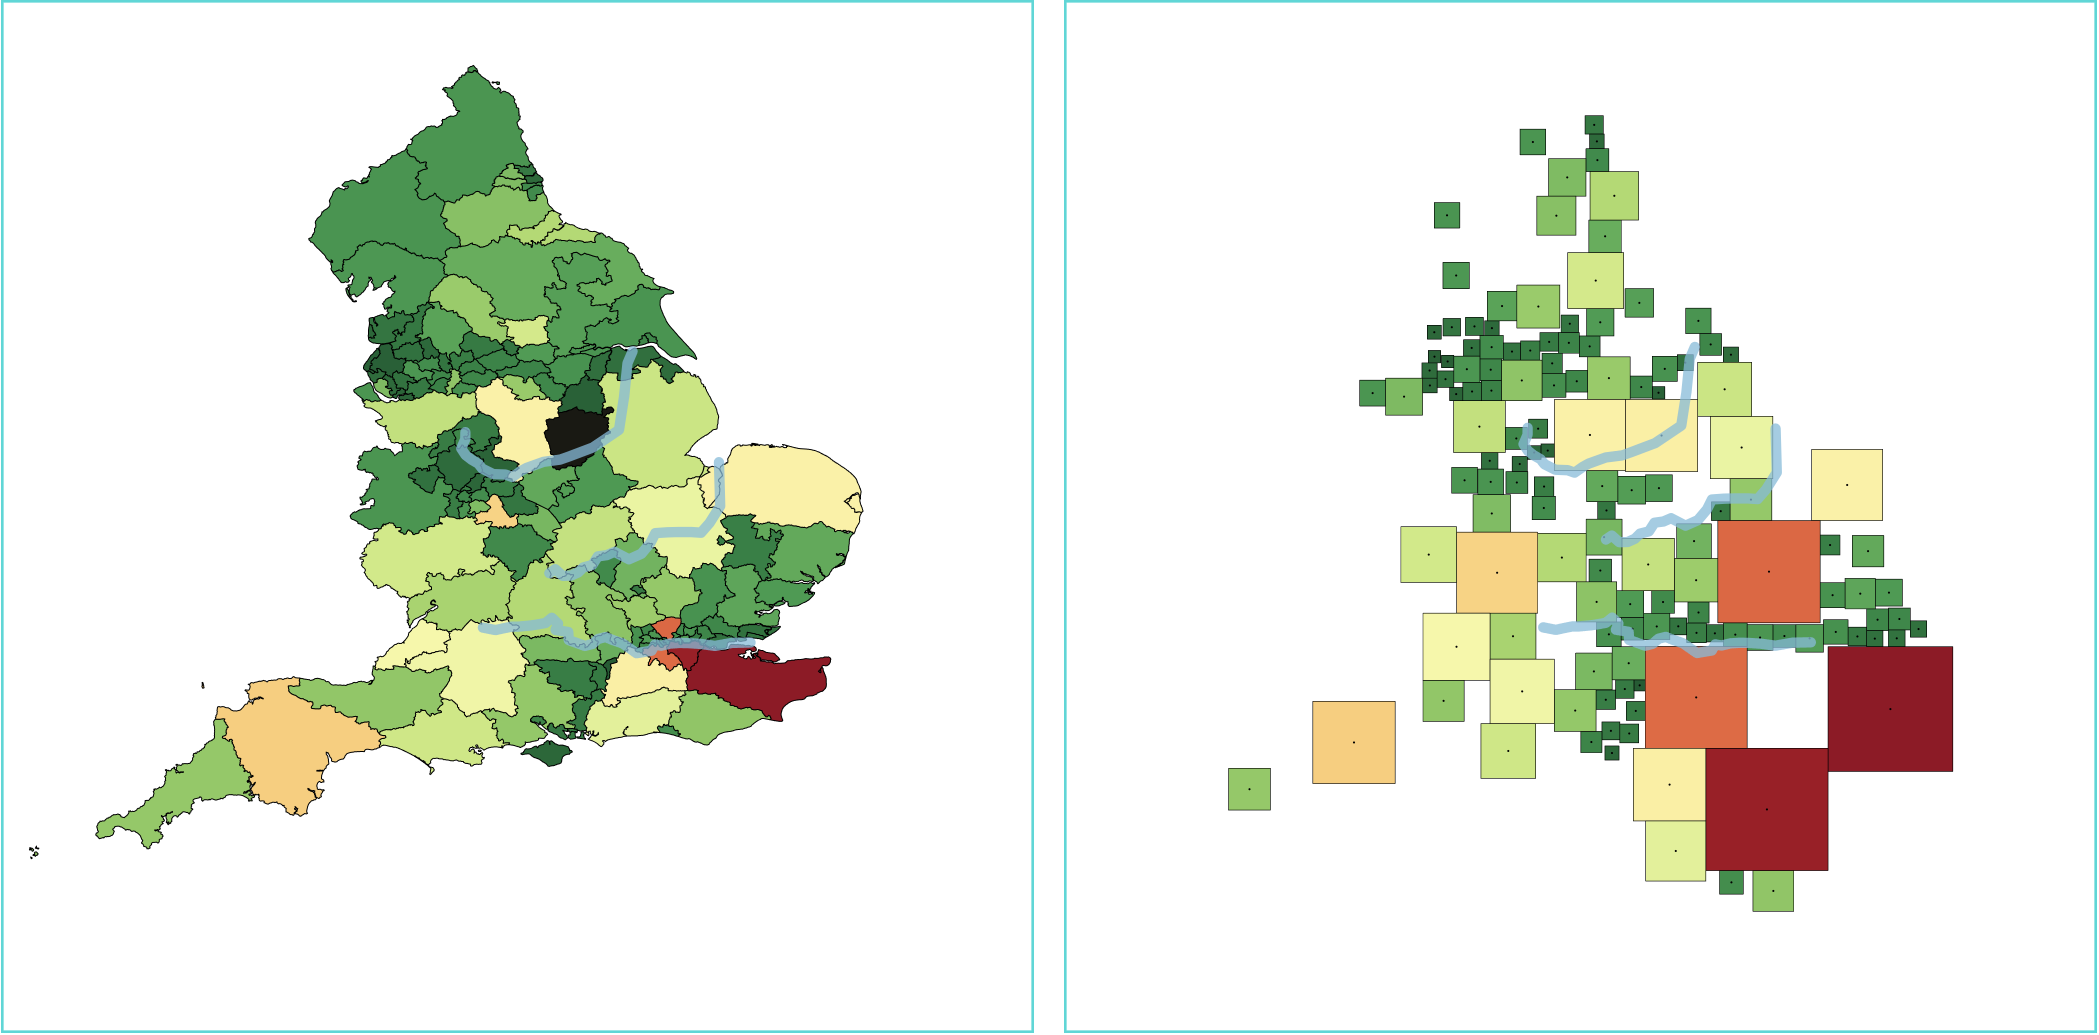
\includegraphics[width=\columnwidth,keepaspectratio]{figure/evaluation/task.png}
            \caption{A sample location task for participants. The left shows the choropleth map, and the right shows the corresponding cartogram. Both images show the three longest rivers in England, and color is mapped to CCG population. The target CCG blinks on the choropleth (shown in black), and participants are asked to identify this CCG on the cartogram. In this figure, $ \nodeCartographicErrorMax $ = 1.875\% , and an $ \nodeTopologicalError $ of 6.67\% is eliminated. }
            \label{fig:task}
        \end{figure}
    }

\subsubsection{Procedure}

The user study is designed to be conducted online, and participants are asked to complete the tasks using their own hardware. The user study includes four parts:

\textbf{P1:} The participants are asked to listen to instructions and training provided as both text and videos. The instructions are designed to help participants understand the concepts used in the tasks. Instructional videos are available at \URL{https://www.youtu.be/playlist?list=PLL7sHvxLtD75fMtrUQrAdddjt3wfFkcWz}.

\textbf{P2:} The participants are given three practice tasks to familiarize themselves with the user study design. These tasks also serve as a quality test to see whether users are taking the study seriously. A demonstration of three sample tasks is also included in the instructional video.

\textbf{P3:} The participants are asked to complete 16 location tasks that involve 4 CCGs. Response and reaction time are recorded. These 4 CCGs are selected to avoid extreme cases (thus bias the result), in terms of size, color, and location.

\textbf{P4:} The participants are asked to complete a questionnaire that consists of Likert Scale questions and open-ended questions.

The materials for P1-P4 are available on the Open Science Foundation website at \URL{https://osf.io/q39w7}.

\subsection{User Study Results}

{
    \begin{figure}[b!]
        \centering
        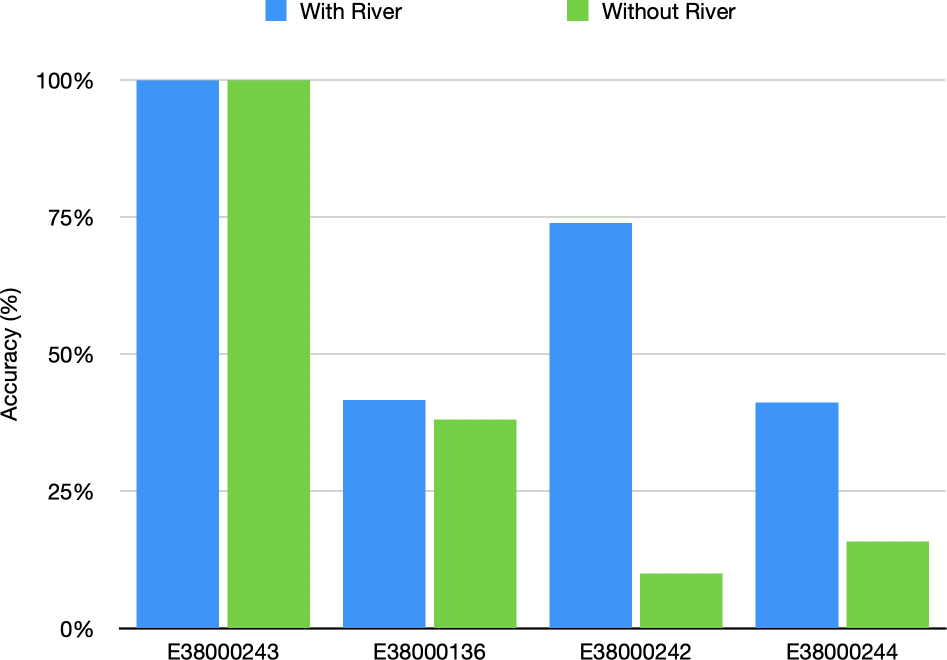
\includegraphics[width=\columnwidth,keepaspectratio]{figure/evaluation/accuracy.png}
        \caption{In the bar chart, the y-axis shows the average accuracy rate of locating CCGs with and without rivers for user study participants. The x-axis shows the target CCGs.}
        \label{fig:task-acc}
    \end{figure}
}


In this section, we analyze the results of our preliminary user study. We recruited \pCount participants to perform 16 location tasks each, in total we collected 384 responses, 24 responses that took over 60 seconds are excluded from the analysis. We hypothesize that participants who took longer than 60 seconds to complete a task were distracted from the study.

\bobgraph{Accuracy:} \Cref{fig:task-acc} shows the accuracy measured by the number of correct CCGs chosen by the participants. The chart shows that the introduction of rivers has improved the accuracy of two CCGs. The accuracy for the two groups differs significantly according to the two-sample unequal variance $t$-test performed, $t$(262.98) = 3.76, $p$ = 0.0002. This supports our hypothesis H1.1 that the introduction of rivers increases target location accuracy.


\bobgraph{Response Time:} \Cref{fig:task-rt} shows the average time to locate a CCG measured for four CCGs. The chart indicates that the introduction of rivers has slightly reduced the time needed to locate CCGs. The two groups show no statistically significant differences according to the two-sample unequal variance $t$-test performed, $t$(356.03) = 0.87, $p$ = 0.38. However, the average time to locate a given CCG is reduced for 3 out of the 4 CCGs users in the study.

    {
        \begin{figure}[t!]
            \centering
            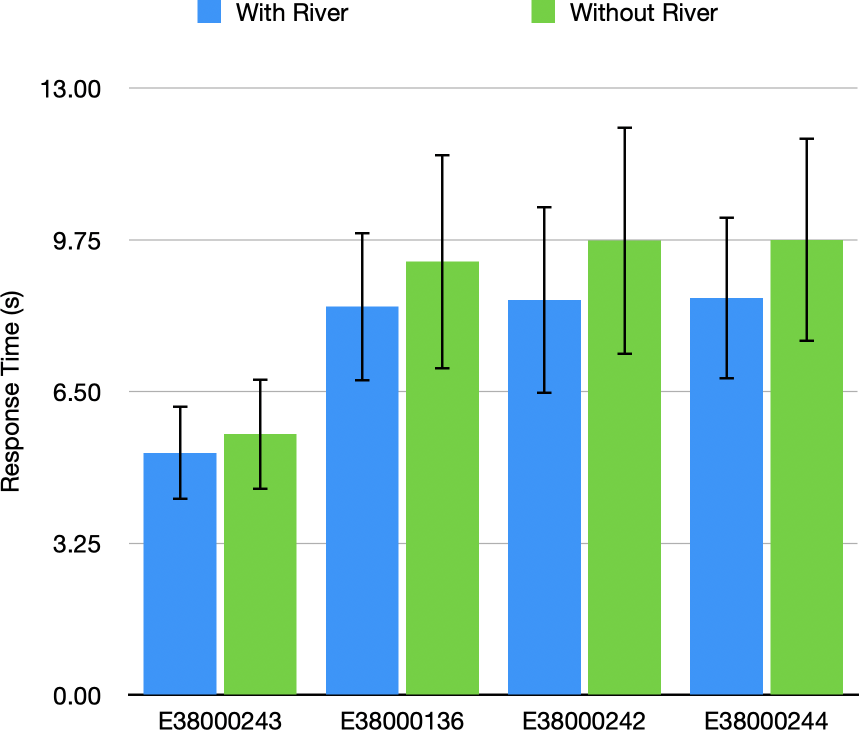
\includegraphics[width=\columnwidth,keepaspectratio]{figure/evaluation/rt.png}
            \caption{In the bar chart, the y-axis shows the average response time for locating CCGs with and without rivers for user study participants. The x-axis shows the target CCGs.}
            \label{fig:task-rt}
        \end{figure}
    }

\bobgraph{Participant Feedback:} \Cref{fig:likert} shows the results of the following Likert Scale questions:
\begin{enumerate}[label=(\Alph*),align=left,leftmargin=*,labelindent=1em]
    \item 87.5\% of participants agree that including rivers is useful.
    \item 83.3\% of participants agree that rivers increase the legibility of a cartogram.
    \item 95.8\% of participants agree that including rivers makes cartograms easier to understand.
    \item 62.5\% of participants agree that including rivers makes CCGs easier to locate.
    \item 87.5\% of participants agree that including rivers adds value to the standard cartogram.
\end{enumerate}

{
\begin{figure}[tb!]
    \centering
    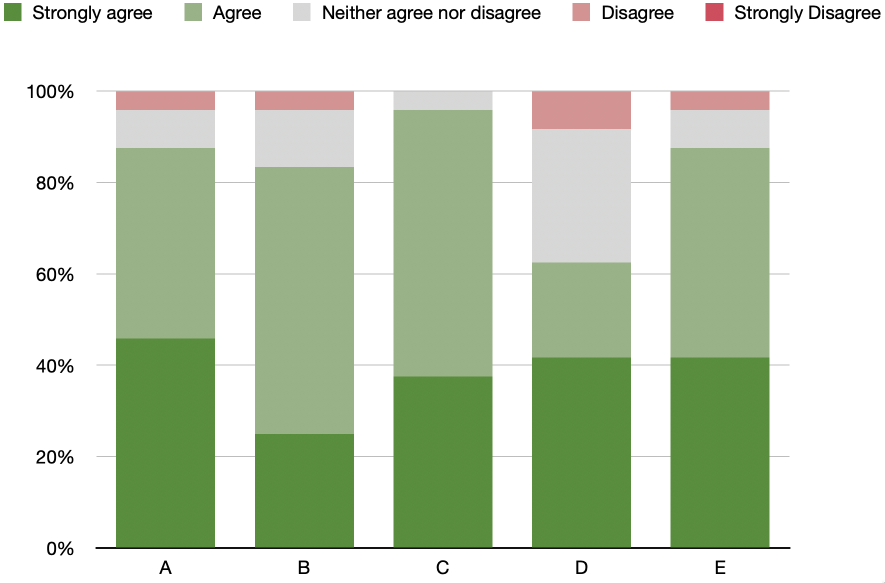
\includegraphics[width=\columnwidth,keepaspectratio]{figure/evaluation/likert.png}
    \caption{The stacked bar chart shows the user study participant responses of Likert Scale questions.}
    \label{fig:likert}
\end{figure}
}

The qualitative results clearly support our hypothesis H1 that rivers generally increase the legibility of cartograms.